\section*{\sffamily \Large NUMERICAL EXAMPLES}
\label{section:sec4}

In this section we present two data analytical scenarios to demonstrate the comparative performance and applicability of the different approaches of robust PCA we have discussed.

{\colrbf 1 more line}

\subsection*{\sffamily \large Bus data}
Available in the R package \texttt{rrcov}, this dataset consists of the measurements of 18 image features for 218 buses. Following a similar analysis in \cite{maronna06}, pp. 213, we set aside variable 9 and scale the other variables by dividing with their respective median absolute deviations (MAD). We do this done because all the variables had much larger standard deviations compared to their MADs, and variable 9 had MAD = 0. Following this, we compare the performances of the classical PCA (CPCA), PCA based on the eigenvector estimate from the MCD covariance matrix (MPCA), spatial sign-based PCA (SPCA), depth-based weighted sign PCA (DPCA), ROBPCA, and PCP.
We use projection depth as our choice of depth function while doing DPCA.

For all classical PCA methods, we set the number of PCs at 3. We compare the above methods using the distance of actual data and their projections on the principal component space. For PCP, these are is simply row norms of the sparse matrix $\bfS_0$ obtained from the procedure, while for other methods this is the orthogonal distances of corresponding samples. Each of its column lists different quantiles of the squared orthogonal distance for a sample point from the hyperplane formed by top 3 PCs estimated by the corresponding method. Table \ref{table:bus_table2} presents the different quantiles of squares of these distances for all the methods. For DPCA, the estimated principal component subspaces are closer to the data than CPCA for more than 90\% of samples, and the distance only becomes larger for higher quantiles. This means that for CPCA, estimated basis vectors of the hyperspace get pulled by extreme outlying points, while the influence of these outliers is very low for DPCA. SPCA and ROBPCA perform very closely in this respect, the percentage of points that have less squared distance than CPCA being between 80\% and 90\% for both of them. This percentage is only 60\% for PCP and 50\% for MPCA, which suggests that the corresponding 3-dimensional subspace estimated by MCD is possibly not an accurate representation of the truth, and there is probably enough noise in the data apart from the low-rank and sparse components estimated by PCP.

%\begin{table}[t]
%\centering
%    \begin{tabular}{c|ccccc}
%    \hline
%    \begin{large} $q$ \end{large} & \multicolumn{5}{c}{Method of PCA}         \\ \cline{2-6}
%    ~                   & CPCA     & SPCA & ROBPCA & MPCA & DPCA \\\hline 
%    1                   & 0.188         & 0.549     & 0.410  & 0.514     & 0.662     \\
%    2                   & 0.084         & 0.272     & 0.214  & 0.337     & 0.359     \\
%    3                   & 0.044         & 0.182     & 0.121  & 0.227     & 0.237     \\
%    4                   & 0.026         & 0.135     & 0.083  & 0.154     & 0.173     \\
%    5                   & 0.018         & 0.099     & 0.054  & 0.098     & 0.115     \\
%    6                   & 0.012         & 0.069     & 0.036  & 0.070     & 0.084     \\ \hline
%    \end{tabular}
%    \caption{Unexplained proportions of variability by PCA models with $q$ components for bus data}
%    \label{table:bus_table1}
%\end{table}

\begin{table}[t]
\centering
    \begin{tabular}{c|cccccc}
    \hline
    Quantile & \multicolumn{6}{c}{Method of PCA}         \\ \cline{2-7}
    ~                   & CPCA     & SPCA & ROBPCA & MPCA & DPCA & PCP\\\hline 
    10\%      & 1.9       & 1.2       & 1.2    & 1.0       & 1.2       & 1.3\\
    20\%      & 2.3       & 1.6       & 1.6    & 1.3       & 1.6       & 1.8\\
    30\%      & 2.8       & 1.8       & 1.8    & 1.7       & 1.9       & 2.1\\
    40\%      & 3.2       & 2.2       & 2.1    & 2.1       & 2.3       & 2.5\\
    50\%      & 3.7       & 2.6       & 2.5    & 3.1       & 2.6       & 3.2\\
    60\%      & 4.4       & 3.1       & 3.0    & 5.9       & 3.2       & 3.8\\
    70\%      & 5.4       & 3.8       & 3.9    & 25.1      & 3.9       & 5.7\\
    80\%      & 6.5       & 5.2       & 4.8    & 86.1      & 4.8       & 11.9\\
    90\%      & 8.2       & 9.0       & 10.9   & 298.2     & 6.9      & 80.2\\
    Max       & 24        & 1037      & 1055   & 1037      & 980      & 1157\\\hline
    \end{tabular}
    \caption{Quantiles of squared data-to-projection distances for bus data}
    \label{table:bus_table2}
\end{table}

\subsection*{\sffamily \large Image denoising}
In this example we take the pixel matrices from four image files: the Lenna image, and three images from the extended Yale Face Database B \citep{GeBeKr01,KCLee05} (fifth images for individuals 1, 2 and 28), add noise to some pixels and attempt to recover the original images using robust PCA techniques. As mentioned before, a major area of application of robust PCA, and PCA in general, is to extract the underlying low-rank structure in image recognition problems that are often high-dimensional in nature. Although PCP was designed keeping this very generative model (i.e. (\ref{eqn:PCPmodel})) in mind, \cite{ZhaoEtal14} showed that even the classical PCA performs fairly well in comparison of low-rank-plus-sparse methods to remove certain types of noise from an image, as well as background subtraction of videos.

\begin{figure}[t]
\centering
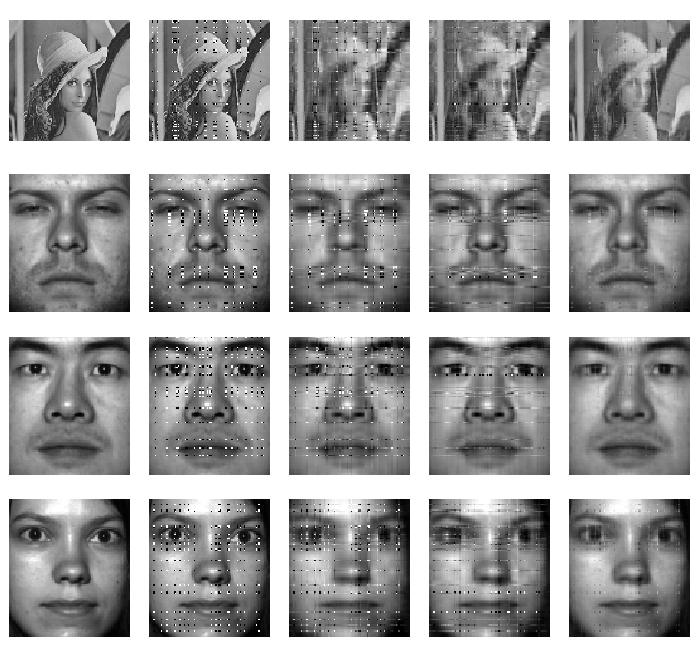
\includegraphics[width=.8\textwidth]{all_denoise}
\caption{Denoising results of four images. Left to right in a row indicates the original image, image with noise added, and denoising by DPCA, ROBPCA and PCP, respectively.}
\label{fig:figDenoise}
\end{figure}

We first resize our images: the lenna image from $128 \times 128$ to $96 \times 96$ and the Yale images from $192 \times 168$ to $96 \times 84$. After this we randomly select 10\% of the pixels from each image and turn their values to 0 or 1 with probability 0.5. Such noise occurs naturally in image recognition problems, and degrades image quality as well as the performance of image classification algorithms \citep{Qiuetal04}. Following this we center and scale each of these matrices of pixel values and apply DPCA, ROBPCA and PCP on them. We take the top 10 estimated PCs for DPCA and ROBPCA to reconstruct the images. Figure~\ref{fig:figDenoise} gives the results obtained from each of these methods. The first and second images in each row denote the original image with and without speckle noise, while the others give denoised versions from the three methods. PCP has the best performance: it recovers the faces almost perfectly, and does better than the other two methods for the Lenna image. The structure in the data seem to have affected the performance of DPCA and ROBPCA, which retain some of the noise in the reconstructed versions. Using a larger number of PCs retains the noises as well. Finally, the performance of all methods suffer when they are applied on the Lenna image, which is a relatively complex image.